% arara: xelatex
\documentclass[12pt]{article}

\usepackage{physics}


\usepackage{tikz} % картинки в tikz
\usepackage{microtype} % свешивание пунктуации

\usepackage{array} % для столбцов фиксированной ширины

\usepackage{indentfirst} % отступ в первом параграфе

\usepackage{sectsty} % для центрирования названий частей
\allsectionsfont{\centering}

\usepackage{amsmath, amsfonts, amssymb} % куча стандартных математических плюшек

\usepackage{comment}

\usepackage[top=2cm, left=1.2cm, right=1.2cm, bottom=2cm]{geometry} % размер текста на странице

\usepackage{lastpage} % чтобы узнать номер последней страницы

\usepackage{enumitem} % дополнительные плюшки для списков
%  например \begin{enumerate}[resume] позволяет продолжить нумерацию в новом списке
\usepackage{caption}

\usepackage{url} % to use \url{link to web}

\usepackage{fancyhdr} % весёлые колонтитулы
\pagestyle{fancy}
\lhead{Time Series and Stochastic Processes}
\chead{}
\rhead{HA}
\lfoot{2023-2024}
\cfoot{}
\rfoot{\thepage/\pageref{LastPage}}
\renewcommand{\headrulewidth}{0.4pt}
\renewcommand{\footrulewidth}{0.4pt}



\usepackage{todonotes} % для вставки в документ заметок о том, что осталось сделать
% \todo{Здесь надо коэффициенты исправить}
% \missingfigure{Здесь будет Последний день Помпеи}
% \listoftodos - печатает все поставленные \todo'шки


% более красивые таблицы
\usepackage{booktabs}
% заповеди из докупентации:
% 1. Не используйте вертикальные линни
% 2. Не используйте двойные линии
% 3. Единицы измерения - в шапку таблицы
% 4. Не сокращайте .1 вместо 0.1
% 5. Повторяющееся значение повторяйте, а не говорите "то же"



\usepackage{fontspec}
\usepackage{polyglossia}

\setmainlanguage{english}
\setotherlanguages{english}

% download "Linux Libertine" fonts:
% http://www.linuxlibertine.org/index.php?id=91&L=1
\setmainfont{Linux Libertine O} % or Helvetica, Arial, Cambria
% why do we need \newfontfamily:
% http://tex.stackexchange.com/questions/91507/
\newfontfamily{\cyrillicfonttt}{Linux Libertine O}

%\AddEnumerateCounter{\asbuk}{\russian@alph}{щ} % для списков с русскими буквами
%\setlist[enumerate, 2]{label=\asbuk*),ref=\asbuk*}

%% эконометрические сокращения
\DeclareMathOperator{\Cov}{\mathbb{C}ov}
\DeclareMathOperator{\Corr}{\mathbb{C}orr}
\DeclareMathOperator{\Var}{\mathbb{V}ar}

\let\P\relax
\DeclareMathOperator{\P}{\mathbb{P}}
\DeclareMathOperator{\plim}{\mathrm{plim}}

\DeclareMathOperator{\E}{\mathbb{E}}
% \DeclareMathOperator{\tr}{trace}
\DeclareMathOperator{\card}{card}
\DeclareMathOperator{\pCorr}{\mathrm{p}\mathbb{C}\mathrm{orr}}


\newcommand \hb{\hat{\beta}}
\newcommand \hs{\hat{\sigma}}
\newcommand \htheta{\hat{\theta}}
\newcommand \s{\sigma}
\newcommand \hy{\hat{y}}
\newcommand \hY{\hat{Y}}
\newcommand \e{\varepsilon}
\newcommand \he{\hat{\e}}
\newcommand \z{z}
\newcommand \hVar{\widehat{\Var}}
\newcommand \hCorr{\widehat{\Corr}}
\newcommand \hCov{\widehat{\Cov}}
\newcommand \cN{\mathcal{N}}
\newcommand \RR{\mathbb{R}}
\newcommand \NN{\mathbb{N}}
\newcommand{\cF}{\mathcal{F}}
\newcommand{\cH}{\mathcal{H}}


\begin{document}

\section*{Home Assignment 1}

\begin{enumerate}
  \item Consider two identical hedgehogs starting at the vertices $A$ and $B$ of a polygon $ABCDE$. 
  Each minute they simulteneously and independently choose to go clockwise or counter-clockwise 
  in the next vertex. 

  The brotherhood of two brave hedgehogs can be in three states: in one vertex, 
  in two adjacent vertices, in two non-adjacent vertices. 

  \begin{enumerate}
    \item What is the probability that they will be in one vertex after 3 steps?
    \item Write down the transition matrix of the brotherhood Markov chain. 
    \item What proportion of time the brotherhood will spend in each state in the long run?
    \item Find the expected time until the hedgehogs meet in one vertex.
  \end{enumerate}
  \item Each day the Random Restaurant is independently closed with probability $p$.
  If the restaurant is open then the number of clients has Poisson distribution with mean $\mu$. 

  After $N$ days (working or non-working) the Random Restaurant will permanently close and you are right, 
  $N$ is random and has Poisson distribution with mean $n$. 


  \begin{enumerate}
    \item Find the moment generating function of the number of clients during day 1, 
    assuming $N \geq 1$. 
    \item Find the moment generating function of the total number of clients served in 
    the Random Restaurant. 
  \end{enumerate}
  
  
  \item Find the probability limit $\plim X_n$, where 
  \[
  X_n = \frac{Y_1 + 2Y_2 + 3Y_3 + \ldots + nY_n}{n^2}
  \]
  and $Y_1$, $Y_2$, \ldots{ } are independent uniform on $[0;1]$. 

  Hint: try to calculate $\E(X_n)$, $\Var(X_n)$.
  You may google the formulas for $1 + 2 + \ldots + n$ and $1^2 + 2^2 + \ldots + n^2$ or ask ChatGPT.
  \item Consider the Poisson arrival process $X_t$ with constant rate $\lambda$. 

  Now let's scale the time in a non-linear fashion, $Y_t = X_{t^2}$.

  \begin{enumerate}
    \item Find $\E(Y_t)$, $\Var(Y_t)$, $\P(Y_t = 0)$.
    \item Find $\E(Y_{t+5} \mid Y_t)$ and $\Var(Y_{t+5} \mid Y_t)$.
  \end{enumerate}

  \item Let's toss a dice until the first six appears. 
  Let $X$ be the result of the first toss and $Y$ — the total number of tosses.

  \begin{enumerate}
    \item Find $\E(X \mid Y)$, $\E(Y \mid X)$.
    \item Find $\Var(X \mid Y)$, $\Var(Y \mid X)$.
  \end{enumerate}

  \item The joint distribution of $X$ and $Y$ is given in the table
    
    \begin{tabular}{*{4}{c}}
    \toprule
    & $X=-1$ & $X=0$ & $X=1$ \\
    \midrule
    $Y=0$ & 0.1 & 0.2 & 0.3  \\
    $Y=1$ & 0.2 & 0.1 & 0.1  \\
    \bottomrule
    \end{tabular}
    
    \begin{enumerate}
     \item Explicitely find the $\sigma$-algebras $\sigma(X)$, $\sigma(Y)$, $\sigma(X \cdot Y)$.
     \item How many elements are there in $\sigma(X, Y)$, $\sigma(X + Y)$, $\sigma(X, Y, X+Y)$?
    \end{enumerate}
    
\end{enumerate}


\newpage
\section*{Home Assignment 2}
Hereinafter $(W_t)$ is a standard Wiener process.  

\begin{enumerate}

  
  \item Some questions about Wiener process!
  \begin{enumerate}
    \item Find $\E(W_7 \mid W_5)$, $\Var(W_7\mid W_5)$, $\E(W_7 W_6 \mid W_5)$.
    \item Find $\E(W_5 \mid W_7)$, $\Var(W_5\mid W_7)$.
  \end{enumerate}
  
  \item Let $(W_t)$ be a standard Wiener process and $Y_t = W_t^3 + t^2 W_t^2$.
  \begin{enumerate}
    \item Find $\E(Y_t)$ and $\Var(Y_t)$.
    \item Is $Y_t$ a martingale?
    \item Find $\E(Y_{t} \mid W_s)$ for $t \geq s$. 
  \end{enumerate}


  \item Consider two independent Wiener processes $A_t$ and $B_t$.
  Check whether these processes are Wiener processes:
  \begin{enumerate}
    \item $X_t = (A_t + B_t) / 2$.
    \item $Y_t = (A_t + B_t) / \sqrt{2}$.
  \end{enumerate}

  \item Using Ito's lemma find $dX$ and the corresponding full form.
  \begin{enumerate}
    \item $X_t = W_t^6 \cos t$.
    \item $X_t = Y_t^3 + t^2 Y_t$ where $dY_t = W_t^2 dW_t + tW_t dt$.
  \end{enumerate}

  \item Consider $I_t = \int_0^t W_u^2 u^2 du$. 
  Find $\E(I_t)$, $\Var(I_t)$ and $\Cov(I_t, W_t)$.

  \item Let $X_t = 42 + t^2W_t^3 + tW_t^2 + \int_0^t 3W_u du + \int_0^t W_u^3 dW_u$.
  \begin{enumerate}
    \item Find $dX_t$.
    \item Is $X_t$ a martingale? Is $Y_t = X_t - \E(X_t)$ a martingale? Provide a short argument for your answer. 
  \end{enumerate}
  
  

\end{enumerate}


\newpage
\section*{Home Assignment 3}
\begin{enumerate}
  
  
  \begin{minipage}{0.42\linewidth}
    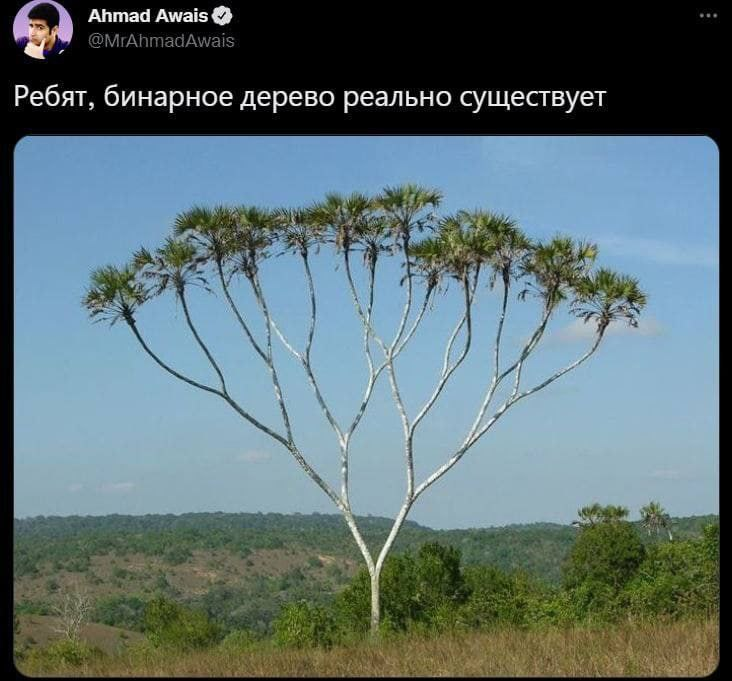
\includegraphics[width=7cm]{tree.jpg}  
  \end{minipage}
  %
  \begin{minipage}{0.58\linewidth}
    \item Consider two-period binomial tree model without dividents.
    Initial stock price is $S_0 = 200$, 
    in each period the stock price is multiplied by $u=1.15$ or by $d=0.75$. 
    One period interest rate is $r=0.05$. 
    
    \begin{enumerate}
    \item Find the risk-neutral probability. 
    \item Price the following binary option: at time $T=2$ you get $100\$ $ if $S_1 > 200$ and nothing otherwise. 
    \item Price the following chooser option: at $t=1$ the owner 
    of the option decides whether the option is call or put. The strike price 
    is $K=200$ and expiry date is $T=2$. 
    \end{enumerate}
    \end{minipage}
  
  
  
  \item In the framework of Black and Scholes model find the price at $t=0$ of the following two 
  financial assets, $dS_t = \mu S_t dt + \sigma S_t dW_t$ is the share price equation. 
  \begin{enumerate}
    \item The asset pays you at time $T$ exactly one dollar if $S_T < K$ where $K$ is a constant 
    specified in the contract. 
    \item The asset pays you at time $T$ exactly $S_T^2$ dollars.
  \end{enumerate}
  
  
  
  \item Consider the Vasicek interest rate model, 
  \[
    dR_t=5(0.06 - R_t) \, dt + 3 \, dW_t, \quad R_0 = 0.07.
  \]
  Here $R_t$ is the interest rate.
  \begin{enumerate}
  \item Using the substitution $Y_t=e^{at} R_t$ find the solution of the stochastic differential equation.
  Start by finding $dY_t$. 
  \item Find $\E(R_t)$ and $\Var(R_t)$.
  \item Which value in this model would you call long-term equilibrium rate and why?
  \end{enumerate}
  
  Hint: you may have integrals in you expression for $R_t$, but no $R_t$.
  
  \item Let $X_t$ be the exchange rate measured in roubles per dollar. 
  We suppose that $dX_t = \mu X_t dt + \sigma X_t dW_t$. 
  
  Consider the inverse exchange rate $Y_t = 1/X_t$ measured in dollars per rouble. 
  
  Write the stochastic differential equation for $dY_t$. 
  The equation may contain $Y_t$ and constants, but not $X_t$.
  
  \item Solve the stochatic differential equation
\[
dY_t = - Y_t dt + dW_t, \; Y_0 = 1
\]

If you are have no clues you may try a substitution $Z_t = f(t) Y_t$. 
Do not forget that the final answer may contain integrals that can't be calculated explicitely. It's ok.




  \end{enumerate}
  


\newpage
\section*{Home Assignment 4}

\begin{enumerate}
  \item The process $(u_t)$ is a white noise with variance $\Var(u_t) = \sigma^2$. 
  Consider the process $b_t = t^2 + 6t + (1-2L)^2 u_t$. %, $b_t = \frac{1}{1-0.3 L}u_t$, $c_t = \frac{1 - 0.3F}{1-0.3L}u_t$, $d_t = \frac{1 - 0.4F}{1-0.3L}u_t$.
  
  \begin{enumerate}
    \item Write explicit expression for $(b_t)$ without lag operator $L$.
    \item Find $\E(b_t)$ and $\Var(b_t)$.
    \item Find $\Cov(b_t, b_{t-k})$ and $\Corr(b_t, b_{t-k})$.
    \item Is the process $(b_t)$ weakly stationary?    
  \end{enumerate}

  \item Let $(u_t)$ be a white noise process with variance $\Var(u_t) = \sigma^2$ and 
  \[
  y_t = 1 + u_t + 0.7u_{t-1} + 0.7^2 u_{t-2} + 0.7^3 u_{t-4} + \ldots  
  \]
  \begin{enumerate}
    \item Find $\E(y_t)$, $\Var(y_t)$.
    \item Find $\Cov(y_t, y_{t-k})$.
    \item Is $(y_t)$ weakly stationary?
    \item Sketch the autocorrelation function of $(y_t)$ if it is weakly stationary.
  \end{enumerate}


  % \item The process $(y_t)$ is weakly stationary with $\gamma_k = \Cov(y_t, y_{t+k})$.
  % Consider the process  $b_{t}=4y_{t} - 3 y_{t-1} + 18$.

  % \begin{enumerate}
  %   \item Find new covariances $\theta_k = \Cov(b_t, b_{t+k})$ in terms of old covariances $(\gamma_j)$.
  %   \item Is $(b_t)$ weakly stationary?
  % \end{enumerate}

  \item Provide an example of two dependent processes $(a_t)$ and $(b_t)$ such that each of them is weakly stationary, 
  but their sum is not weakly stationary. 


  \item Consider three variables $(y_1, y_2, y_3)$ that are jointly normal
  \[
  y \sim \cN\left( \begin{pmatrix}
    2 \\
    6 \\
    11 \\
  \end{pmatrix}; \begin{pmatrix}
    16 & 0 & -1 \\
    0 & 4 & 1 \\
    -1 & 1 & 4 \\
  \end{pmatrix}  \right).  
  \]

  Find $\Corr(y_1, y_2)$ and partial correlation $\pCorr(y_1, y_2 ; y_3)$.

  \item Let $y_t = 5 + u_t + u_{t-1} + u_{t-2}$ where $(u_t)$ is a white noise with variance $\Var(u_t) = \sigma^2$.
  \begin{enumerate}
    \item Is the process $(y_t)$ weakly stationary?
    \item Find the autocorrelation function $\rho_k$ for this process. 
    \item Find the first two values of the partial autocorrelation function, $\phi_{11}$ and $\phi_{22}$.
  \end{enumerate}

  \item {[bonus]} Variables $u_1$ and $u_2$ are independent $\cN(0;1)$. 
  Consider the process $y_t = u_1 \cos (\pi t /2) + u_2 \sin (\pi t /2)$.

  \begin{enumerate}
    \item Find $\E(y_t)$, $\Var(y_t)$, $\gamma_k = \Cov(y_t, y_{t+k})$. 
    \item Is $(y_t)$ weakly stationary? 
    \item Can $(y_t)$ be represented as $MA(\infty)$ process with respect to \textit{some} white noise, not necessary $(u_t)$?
  \end{enumerate}

  Your know additionally that $y_{100} = 0.2024$. 
  \begin{enumerate}[resume]
    \item What is your best point prediction for $y_{104}$? 
    \item What is the shortest prediction interval that covers $y_{104}$ with at least 95\%-probability?
  \end{enumerate}


\end{enumerate}





\end{document}

\begin{enumerate}

  \item Consider the Markov chain with the transition matrix
  
  \[
    P = \begin{pmatrix}
      0.2   & 0.8 \\
      0.7 & 0.3 \\
    \end{pmatrix}.
  \]
  The hedgehog starts at the first state and moves randomly according to transition matrix $P$.

  \begin{enumerate}
    \item Draw the graph of this chain. 
    \item What is the probability that the hedgehog will be in state 2 after 3 moves?
    \item What is the stationary distribution of this chain?
  \end{enumerate}

  \item Consider iid sequence $X_1$, $X_2$, \ldots~of uniform on $[0;10]$ random variables. 
  Find the following probability limits:
  \[
   L_1 = \plim \frac{X_1 + X_2 + \ldots + X_n}{2n}, \; L_2 = \plim \frac{X_1^2 + X_2^2 + \ldots + X_n^2}{X_1 + X_2 + \ldots + X_n}, \;
   L_3 = \plim (X_1 \cdot X_2 \cdot \ldots \cdot  X_n)^{1/n}.
  \]

   Hint: maybe there is a function that can transform the product $L_3$ into the sum? 
   you are free to use any probability limit property. 

   \item Consider iid sequence $X_1$, $X_2$, \ldots~of uniform on $[0;10]$ random variables. 
   \begin{enumerate}
     \item Find the probability $\P(\abs{\max\{X_1, X_2, \ldots, X_n\} - 10} > \varepsilon)$.
     \item Find the probability limit $\plim \max\{X_1, X_2, \ldots, X_n\}$ by definition. 
   \end{enumerate}
   
  \item Joe Biden throws a die until six or five appears.
  For every throw he pays $0.1$ dollars, but at the end he receives the result of the last throw in dollars.
  

\begin{enumerate}
  \item What is the expected payoff of Joe?
  \item Assume now that Joe can stop the game at every moment of time. 
  
  What is the maximal expected payoff and the corresponding strategy?
\end{enumerate}


\item Ilya Muromets stands before the first stone. There are three roads behind the stone. 
And every road ends with a new stone. And there are three new roads behind every new stone. And so on. 
Every road is guarded with one-third probability by a three headed dragon Zmei Gorynich.
Yes, there are infinitely many Zmeis Gorynichs.

\begin{enumerate}
\item What is the probability that Ilya will never meet Zmei Gorynich if Ilya chooses a road at random?
\item What is the probability that Ilya will meet Zmei Gorynich after passing by even number of stones
if Ilya chooses a road at random?
\item What is the probability that \textbf{there exists} at least one Eternal Peaceful Path without Zmei Gorynich?
\end{enumerate}


\end{enumerate}

Deadline: \textbf{2022-10-02, 21:00}. 

\newpage

\section*{Home Assignment 2}

Hereinafter $(W_t)$ is a standard Wiener process.  

\begin{enumerate}

  
  \item Some questions about Wiener process!
  \begin{enumerate}
    \item Find $\E(W_7 \mid W_5)$, $\Var(W_7\mid W_5)$, $\E(W_7 W_6 \mid W_5)$.
    \item Find $\E(W_5 \mid W_7)$, $\Var(W_5\mid W_7)$.
  \end{enumerate}
  
  \item Using Ito's lemma find $dX$ and the corresponding full form.
  \begin{enumerate}
    \item $X_t = W_t^6 \cos t$.
    \item $X_t = Y_t^3 + t^2 Y_t$ where $dY_t = W_t^2 dW_t + tW_t dt$.
  \end{enumerate}

  %\item Consider a standard Wiener process $(W_t)$.
  %\begin{enumerate}
  %  \item Find the expected value $M(u) = \E(\exp(u W_t))$. It's called moment generating function :)
  %  \item What is the probabilistic meaning of $M'''(0)$?
  %  
  %  Hint: you may interchange expected value and derivative without proof. 
  %  \item Using the Taylor expansion for $M(u)$ find at once all the expected values of $\E(W_t^k)$ for $k\in \mathbb N$.
  %  
  %  Hint: 
  %  \[
  %  \exp(a) = 1 + a + \frac{a^2}{2!} + \frac{a^3}{3!} + \ldots  = f(0) + f'(0) a + \frac{f''(0)}{2!}a^2 + \frac{f'''(0)}{3!}a^3 +  \ldots
  %  \]
  % \end{enumerate}

  \item Consider two independent Wiener processes $A_t$ and $B_t$.
  Check whether these processes are Wiener processes:
  \begin{enumerate}
    \item $X_t = (A_t + B_t) / 2$.
    \item $Y_t = (A_t + B_t) / \sqrt{2}$.
  \end{enumerate}

  \item Consider $I_t = \int_0^t W_u^2 u^2 du$. 
  Find $\E(I_t)$, $\Var(I_t)$ and $\Cov(I_t, W_t)$.


  \item Find limits in $L^2$ of the following sequences for $n\to \infty$:
  \begin{enumerate}
%    \item Non-stochastic one first:
%    \[
%      R_n = \sum_{i=1}^n \left(h(it/n) - h((i-1)t/n)\right)^2, \text{ where } h(u) = 3u^2.
%    \]
    \item 
    \[
    S_n = \sum_{i=1}^n (t/n)\left(W(it/n) - W((i-1)t/n)\right).
    \]
    \item 
    \[
      T_n = \sum_{i=1}^n \left(W(it/n) - W((i-1)t/n)\right)^5.
    \]
  \end{enumerate}
  

  \item (bonus) Let's split the time segment $[0;10]$ into $n=10^5$ sub-segments of equal lentgh. 
  Let $\Delta_i$ be equal to the corresponding increment of Wiener process, 
  $\Delta_i = W(10i/n) - W(10(i-1)/n)$. 
   \begin{enumerate}
     \item What is the distribution of $\Delta_i$?
     \item Using any open source software simulate five approximate trajectories of Wiener process and plot them 
     on the same plot. You can generate $\Delta_i$ and find a cumulative sum. 
     \item Now simulate $n_{sim} = 10^4$ trajectories but do not plot them. 
     Using these trajectories estimate the probability $p = \P(\max_{t \in [0;10]}W_t > 7)$. 
   \end{enumerate}
   
   Do not forget to provide your code. 
 

\end{enumerate}


Deadline: \textbf{2022-12-06, 21:00}. 



\newpage

\section*{Home Assignment 3}

\begin{enumerate}
\item Let $X_t = 42 + t^2W_t^3 + tW_t^2 + \int_0^t 3W_u du + \int_0^t W_u^3 dW_u$.
\begin{enumerate}
  \item Find $dX_t$.
  \item Is $X_t$ a martingale? Is $Y_t = X_t - \E(X_t)$ a martingale? 
\end{enumerate}

Hint: only the binary answer for (b) is not sufficient but the argument is very-very short if you solve (a). 



\begin{minipage}{0.42\linewidth}
  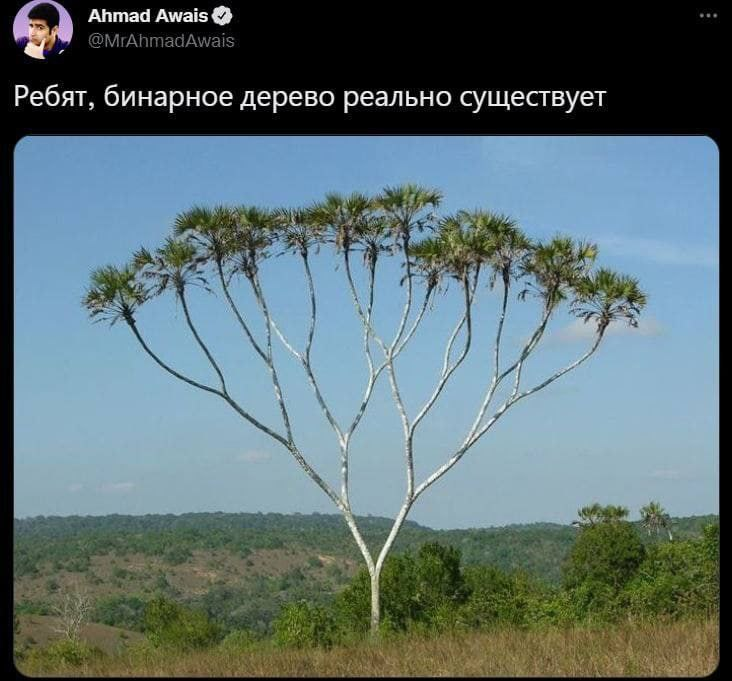
\includegraphics[width=7cm]{tree.jpg}  
\end{minipage}
%
\begin{minipage}{0.58\linewidth}
  \item Consider two-period binomial tree model without dividents.
  Initial stock price is $S_0 = 200$, 
  in each period the stock price is multiplied by $u=1.15$ or by $d=0.75$. 
  One period interest rate is $r=0.05$. 
  
  \begin{enumerate}
  \item Find the risk-neutral probability. 
  \item Price the following binary option: at time $T=2$ you get $100\$ $ if $S_1 > 200$ and nothing otherwise. 
  \item Price the following chooser option: at $t=1$ the owner 
  of the option decides whether the option is call or put. The strike price 
  is $K=200$ and expiry date is $T=2$. 
  \end{enumerate}
  \end{minipage}



\item In the framework of Black and Scholes model find the price at $t=0$ of the following two 
financial assets, $dS_t = \mu S_t dt + \sigma S_t dW_t$ is the share price equation. 
\begin{enumerate}
  \item The asset pays you at time $T$ exactly one dollar if $S_T < K$ where $K$ is a constant 
  specified in the contract. 
  \item The asset pays you at time $T$ exactly $S_T^2$ dollars.
\end{enumerate}



\item Consider the Vasicek interest rate model, 
\[
  dR_t=5(0.06 - R_t) \, dt + 3 \, dW_t, \quad R_0 = 0.07.
\]
Here $R_t$ is the interest rate.
\begin{enumerate}
\item Using the substitution $Y_t=e^{at} R_t$ find the solution of the stochastic differential equation.
Start by finding $dY_t$. 
\item Find $\E(R_t)$ and $\Var(R_t)$.
\item Which value in this model would you call long-term equilibrium rate and why?
\end{enumerate}

Hint: you may have integrals in you expression for $R_t$, but no $R_t$.

\item Let $X_t$ be the exchange rate measured in roubles per dollar. 
We suppose that $dX_t = \mu X_t dt + \sigma X_t dW_t$. 

Consider the inverse exchange rate $Y_t = 1/X_t$ measured in dollars per rouble. 

Write the stochastic differential equation for $dY_t$. 
The equation may contain $Y_t$ and constants, but not $X_t$.


\end{enumerate}


Deadline: \textbf{2022-12-18, 21:00}. 

\section*{Home Assignment 4: stationarity, white noise, MA model}
\begin{enumerate}
  \item The process $(u_t)$ is a white noise. 
  Consider the processes $a_t = (1+L)^3 u_t$ and 
  $b_t = t^2 + 6t + (1-2L)^2 u_t$. %, $b_t = \frac{1}{1-0.3 L}u_t$, $c_t = \frac{1 - 0.3F}{1-0.3L}u_t$, $d_t = \frac{1 - 0.4F}{1-0.3L}u_t$.
  
  \begin{enumerate}
    \item Write explicit expression of these processes without lag $L$ operator.
    \item Check whether these processes are stationary.
    \item For stationary processes find the autocorrelation function. 
    \item Check whether these processes are white noises.
    \item If the process is $MA(k)$ process with respect to $(u_t)$ then find the value of $k$.  
    
  \end{enumerate}

  \item The process $(y_t)$ is stationary with $\gamma_k = \Cov(y_t, y_{t+k})$.
  Consider the process  $b_{t}=4y_{t} - 3 y_{t-1} + 18$.

  \begin{enumerate}
    \item Find new covariances $\theta_k = \Cov(b_t, b_{t+k})$ in terms of old covariances $(\gamma_j)$.
    \item Is $(b_t)$ stationary?
  \end{enumerate}

  \item Provide an example of two dependent processes $(a_t)$ and $(b_t)$ such that each of them is stationary, 
  but their sum is not stationary. 


  \item Consider three variables $(y_1, y_2, y_3)$ that are jointly normal
  \[
  y \sim \cN\left( \begin{pmatrix}
    5 \\
    6 \\
    11 \\
  \end{pmatrix}; \begin{pmatrix}
    9 & 0 & -1 \\
    0 & 4 & 1 \\
    -1 & 1 & 4 \\
  \end{pmatrix}  \right).  
  \]

  Find $\Corr(y_1, y_2)$ and $\pCorr(y_1, y_2 ; y_3)$.


  \item (bonus) Variables $u_1$ and $u_2$ are independent $\cN(0;1)$. 
  Consider the process $y_t = 7 + u_1 \cos (\pi t /2) + u_2 \sin (\pi t /2)$.

  \begin{enumerate}
    \item Find $\E(y_t)$, $\Var(y_t)$, $\gamma_k = \Cov(y_t, y_{t+k})$. 
    \item Is $(y_t)$ stationary? Is it a white noise process?
    \item Your know that $y_{100} = 0.2023$. What is your best prediction for $y_{104}$? What about predictive interval?
    \item Is this process $MA(\infty)$ process with respect to \textit{some} white noise, not necessary $(u_t)$?
  \end{enumerate}
  

\end{enumerate}

Deadline: \textbf{2023-02-12, 21:00}. 


\newpage

\section*{Home Assignment 5: recurrence equations, AR-model, ACF/PACF}
\begin{enumerate}
  \item Consider the recurrence equation $y_t = 4 + 10 y_{t-1} + u_t$ where $(u_t)$ is the white noise.
  \begin{enumerate}
    \item Find two non-stationary solution.
    \item Find one stationary solution. Does this solution have $MA(\infty)$ form with respect to $(u_t)$?
  \end{enumerate}

  \item Consider two equations (A) $y_t = 4 + 0.6 y_{t-1} + 0.2y_{t-2} + u_t$ and (B) $y_t = 3 + y_{t-1} + 6y_{t-2} + u_t$.
  
  \begin{enumerate}
    \item How many non-stationary solutions does each equation have?
    \item How many stationary solutions does each equation have?
    \item How many stationary solutions that are $MA(\infty)$ with respect to $(u_t)$ does each equation have?
  \end{enumerate}

  \item For $MA(2)$ process $y_t = 5 + u_t + 3u_{t-2}$ find all values of the autocorrelation function $\rho_k$ and 
  first two values of the partial autocorrelation function $\phi_{kk}$.

  \item For stationary $AR(1)$ process with equation $y_t = 5 + 0.3y_{t-1} + u_t$ find all values of the autocorrelation function $\rho_k$ and 
  all values of the partial autocorrelation function $\phi_{kk}$.

  \item For stationary $AR(2)$ process with equation $y_t = 5 + 0.3y_{t-1} - 0.02 y_{t-2} + u_t$ find first two values of the autocorrelation function $\rho_k$ and 
  all values of the partial autocorrelation function $\phi_{kk}$.

  \item (bonus) Consider the process 
  \[
  y_t = \frac{1-0.7F}{1-0.7L} u_t,
  \]
  where $(u_t)$ is a white noise and $F$ is the forward operator. 
  \begin{enumerate}
    \item Write explicit expression for $(y_t)$ without lag nor forward operator.
    \item Is $(y_t)$ a white noise?
  \end{enumerate}
\end{enumerate}

Deadline: \textbf{2023-02-19, 21:00}. 

\end{document}

\newpage

\section*{Home Assignment 6: prediction, estimation}
\begin{enumerate}
  \item Consider $AR(1)$


  \item Masha has five observations: $y_1 = 5$, $y_2 = 4$, $y_3 = 7$, $y_4 = 9$, $y_5 = 8$.
  
  Masha assumes the model $y_t = \mu + u_t$, $u_t \sim \cN(0;\sigma^2)$ and independent. 
  Estimate the parameters of Masha's model using unconditional maximum likelihood, 
    \[
      \ln f(y_1, \ldots, y_5) \to \max.
    \]

    \item Sasha has five observations: $y_1 = 5$, $y_2 = 4$, $y_3 = 7$, $y_4 = 9$, $y_5 = 8$.

  Sasha assumes the model $y_t = \mu + y_{t-1} + u_t$, $u_t \sim \cN(0;\sigma^2)$ and independent. 

  Estimate the parameters of Sasha's model using conditional maximum likelihood, 
    \[
      \ln f(y_2, \ldots, y_5 \mid y_1) \to \max.
    \]



  \item Consider two equations (A) $y_t = 4 + 0.6 y_{t-1} + 0.2y_{t-2} + u_t$ and (B) $y_t = 3 + y_{t-1} + 6y_{t-2} + u_t$.
  
  \begin{enumerate}
    \item How many non-stationary solutions does each equation have?
    \item How many stationary solutions does each equation have?
    \item How many stationary solutions that are $MA(\infty)$ with respect to $(u_t)$ does each equation have?
  \end{enumerate}

  \item For $MA(2)$ process $y_t = 5 + u_t + 3u_{t-2}$ find all values of the autocorrelation function $\rho_k$ and 
  first two values of the partial autocorrelation function $\phi_{kk}$.

  \item For stationary $AR(1)$ process with equation $y_t = 5 + 0.3y_{t-1} + u_t$ find all values of the autocorrelation function $\rho_k$ and 
  all values of the partial autocorrelation function $\phi_{kk}$.

  \item For stationary $AR(2)$ process with equation $y_t = 5 + 0.3y_{t-1} - 0.02 y_{t-2} + u_t$ find first two values of the autocorrelation function $\rho_k$ and 
  all values of the partial autocorrelation function $\phi_{kk}$.

  \item (bonus) Consider the process 
  \[
  y_t = \frac{1-0.7F}{1-0.7L} u_t,
  \]
  where $(u_t)$ is a white noise and $F$ is the forward operator. 
  \begin{enumerate}
    \item Write explicit expression for $(y_t)$ without lag nor forward operator.
    \item Is $(y_t)$ a white noise?
  \end{enumerate}
\end{enumerate}


\end{document}





\end{document}


  
  \end{enumerate}
  

\end{enumerate}


Deadline: \textbf{2021-12-04, 21:00}. 






\newpage

\section*{Home Assignment 3}

\begin{enumerate}
\item Let $X_t = 42 + t^2W_t^3 + tW_t^2 + \int_0^t 3W_u du + \int_0^t W_u^3 dW_u$.
\begin{enumerate}
  \item Find $dX_t$.
  \item Is $X_t$ a martingale? Is $Y_t = X_t - \E(X_t)$ a martingale? 
\end{enumerate}

Hint: only the binary answer for (b) is not sufficient but the argument is very-very short if you solve (a). 

\item Consider $I_t = \int_0^t W_u^2 u^2 dW_u$. 

\begin{enumerate}
  \item Find $dI_t$, $\E(I_t)$, $\Var(I_t)$ and $\Cov(I_t, W_t)$.
  \item Find $\E(I_5 \mid I_3)$.
\end{enumerate}


\item In the framework of Black and Scholes model find the price at $t=0$ of the following two 
financial assets, $dS_t = \mu S_t dt + \sigma S_t dW_t$ is the share price equation. 
\begin{enumerate}
  \item The asset pays you at time $T$ exactly one dollar if $S_T < K$ where $K$ is a constant 
  specified in the contract. 
  \item The asset pays you at time $T$ exactly $S_T^2$ dollars.
\end{enumerate}



\item Consider the Vasicek interest rate model, 
\[
  dR_t=5(0.06 - R_t) \, dt + 3 \, dW_t, \quad R_0 = 0.07.
\]
Here $R_t$ is the interest rate.
\begin{enumerate}
\item Using the substitution $Y_t=e^{at} R_t$ find the solution of the stochastic differential equation.
Start by finding $dY_t$. 
\item Find $\E(R_t)$ and $\Var(R_t)$.
\item Which value in this model would you call long-term equilibrium rate and why?
\end{enumerate}

Hint: you may have integrals in you expression for $R_t$, but no $R_t$.

\item Let $X_t$ be the exchange rate measured in roubles per dollar. 
We suppose that $dX_t = \mu X_t dt + \sigma X_t dW_t$. 

Consider the inverse exchange rate $Y_t = 1/X_t$ measured in dollars per rouble. 

Write the stochastic differential equation for $dY_t$. 
The equation may contain $Y_t$ and constants, but not $X_t$.


\end{enumerate}


Deadline: \textbf{2021-12-12, 21:00}. 

\newpage





\item Let $(y_t)$ be a stationary process with autocovariance function $\gamma_k = 20 \cdot 0.5^k$ and expected value $100$. 
  You remove all odd observations and hence your have a new process $z_t = y_{2t}$. 

  \begin{enumerate}
    \item Is the new process $(z_t)$ stationary?
    \item Draw the autocorrelation function of $(z_t)$ if it is stationary. 
  \end{enumerate}



\section*{Home Assignment 2}

\begin{enumerate}


  \item Consider the Markov chain with the transition matrix $P$:
  
  \[
    \begin{pmatrix}
      0.2   & 0.1 & 0.7 &   0 &   0 &   0 &   0  &  0 \\
      0.4 & 0.6 & 0   &   0 &   0 &   0 &   0  &  0 \\
      0   & 0   & 0   &   0.3 &   0 &   0 &   0  &  0.7 \\
      0   & 0 & 0.3 &   0 &   0.7 &   0 &   0  &  0 \\
      0   & 0 & 0 &   0 &   0 &   1 &   0  &  0 \\
      0   & 0 & 0 &   0 &   0 &   0 &   1  &  0 \\
      0   & 0 & 0 &   0 &   0 &   0.4 &   0  &  0.6 \\
      0   & 0 & 0 &   0 &   0 &   1 &   0  &  0 \\
    \end{pmatrix}  
  \]
  
  
  \begin{enumerate}
    \item Draw the most beautiful graph for this chain. A fox or a cat is ok :)
    \item Split the chaininto classes and classify them as closed and not closed.
    \item Classify the states as recurrent and transient.
    \item Find $P^{2022}$ approximately. 
  \end{enumerate}

  \item The Lonely Queen is standing on the B2 field of the chessboard. 
  She starts moving randomly according to chess rules. 

  \begin{enumerate}
    \item Classify the states as recurrent or transient. 
    \item What proportion of her eternal life will the Queen spend on every field?
    \item How many moves on average will it take to go back to B2?
  \end{enumerate}




  \item Ilya and Zmei finally met and play with a coin. 
They throw a coin until the sequence HTH or TTH apears. 
Ilya wins if HTH appears and Zmei wins if TTH appears.

\begin{enumerate}
  \item What is the probability that Ilya wins?
  \item What is the expected number of throws?
  \item What is the expected number of throws given that Ilya won?
\end{enumerate}




\end{enumerate}

Deadline: \textbf{2021-10-09, 21:00}. 




\begin{enumerate}
  \item I walk in the street during the first snow. Snowflakes falling into my palm 
  is a Poisson process with rate $\lambda = 10$ snowflakes per minute.

  \begin{enumerate}
    \item What is the probability that there will be exactly 4 snowflakes in 30 seconds?
    \item What is the expected value and variance of snowflakes in 2 minutes?
  \end{enumerate}

  \item Grasshoppers are scattered accross a field according to a Poisson process with rate one grasshopper per two square meters. 
  
  Which area should I search to find at least one grasshopper with probability $0.9$?

  \item Ilon Mask has two mobile phones. The calls to the first phone are a Poisson process 
  with rate $\lambda_1$, the calls to the second one — a Poisson process with rate $\lambda_2$. 
  Rate is measured in calls per hour. 
  These processes are independent.

  Ilon turns on the phones simulteneously. 
  
  \begin{enumerate}
    \item What is the probability that he receives exactly 2 calls on the first phone and exactly 
    3 calls on the second in one hour? Ilon Mask is like Bruce Willis and can answer unlimited 
    number of calls simulteneously. 
    \item What is covariance between the total number of calls in the first hour and the total 
    number of calls in the first two hours?
    \item (harder) What is the probability that the first phone will ring first?
  \end{enumerate}
  
  Hint: there are at least two ways to solve the hard point. 
  You can calculate a double integral 
  for exponentially distributed waiting times. 
  You can use the assumptions of Poisson process and first step approach.

  \item I wait on the bus stop. The buses arrive according a Poisson process with rate 2 per hour. 
  The taxis arrive according to a Poisson process with rate 5 per hour.  
  
  \begin{enumerate}
    \item What is the probability that at least two taxis will arrive before a bus?
    \item What is the probability that exactly two taxis will arrive before a bus?
  \end{enumerate}
  
  Hint: in this problem you may use the following fact without a proof. For two independent exponentially 
  distributed variables with rates $\lambda_1$ and $\lambda_2$: $\P(Y_1 < Y_2) = \lambda_1 / (\lambda_1 + \lambda_2)$.

  \item (harder) Students arrive to the Grusha caffé according to a Poisson process with rate $\lambda$.
  The service time are independent and exponentially distributed with rate $\mu > \lambda$.

  Let's denote by $S_t$ the number of students in the queue at time $t$ (counting the student who is serviced).
  Imagine that Grusha is open 24/24 and the arrivals and service go on and go on. 
  The distribution of $S_t$ will stabilize, you don't need to prove it. 

  Find the probability $\P(S_t = k)$ for big value of $t$. 


\end{enumerate}

Deadline: \textbf{2021-10-29, 21:00}. 


\newpage

\section*{Home Assignment 3}

\begin{enumerate}
  \item Let $\Omega = \RR$. Explicitely find the sigma-algebras $\cF_1 = \sigma(A)$, $\cF_2 = \sigma(B)$, $\cF_3 = \sigma(A, B)$ where $A=[-10;5]$ and $B=(0;10)$.
  \item I throw a die once. Let $X$ be the result of the toss. 
  Count the number of events in sigma-algebras $\cF_1 =\sigma (X)$, $\cF_2 = \sigma (\{X>3\})$, $\cF_3 = \sigma (\{X > 3\}, \{X<5\})$.

  \item Let $\Omega = \RR$. The sigma-algebra $\cF$ is generated by all the sets of the form $(-\infty, t]$,
  \[
  \cF = \sigma \left( \{ (-\infty; t] \mid t \in \RR\} \right)  
  \]
  Check whether $A_1 = (0; 10) \in \cF$, $A_2 = \{5\} \in \cF$, $A_3 = \NN \in \cF$. 

  \item Prove the following statements or provide a counter-example:
  \begin{enumerate}
    \item If $\cF_1$ and $\cF_2$ are sigma-algebras then $\cF = \cF_1 \cup \cF_2$ is sigma-algebra.
    \item If $X$ and $Y$ are independent random variables then $\card \sigma(X, Y) = \card \sigma(X) + \card \sigma(Y)$.
  \end{enumerate}

  For finite sets $\card$ denotes just the number of elements.

  \item I throw a coin infinite number of times. 
  Let the random variable $X_n$ be equal to $1$ if the $n$-th toss is head and $0$ otherwise. 
  Consider a pack of sigma-algebras: $\cF_n = \sigma (X_1, \ldots, X_n)$ and $\cH_n = \sigma (X_n, X_{n+1}, X_{n+2}\, \ldots)$.

  Where possible provide and example of a non-trivial event (neither $\Omega$ nor $\emptyset$) such that 
  \begin{enumerate}
    \item $A_1 \in \cF_{2020}$;
    \item $A_2 \in \cH_{2020}$;
    \item $A_3 \in \cF_{2020}$ and $A_3 \in \cH_{2020}$;
    \item $A_4 \in \cF_n$ for all $n$; 
    \item $A_5 \in \cH_n$ for all $n$.
  \end{enumerate}

\end{enumerate}


Deadline: \textbf{2021-11-08, 21:00}. 


\newpage

\section*{Home Assignment 4}

\begin{enumerate}

  \item The random variables $Z_n$ are independent and identically distributed with probabilities $\P(Z_n = 1) = 0.2$, 
  $\P(Z_n = -1) = 0.8$. 
  \begin{enumerate}
    \item Find a constant $\alpha$ such that $A_t = \sum_{n=1}^t Z_n - \alpha t$ is a martingale.
    \item Find all constants $\beta$ such that $B_t = \beta^{\sum_{n=1}^t Z_n}$ is a martingale.
  \end{enumerate}


  \item Consider two classes of random processes in discrete time:
  \begin{itemize}
    \item Markov chains, $\P(X_{n+1} = k \mid X_{n}, X_{n-1}, \ldots, X_1) = \P(X_{n+1} = k \mid X_{n})$ for all $n$.
    \item Martingales, $\E(X_{n+1} \mid X_{n}, X_{n-1}, \ldots, X_1 ) = X_n$ for all $n$.
    % \item Stationary processes, $\E(X_n) = \mu$, $\Cov(X_n, X_{n-k}) = \gamma_k$ for all $n$ and $k$.
  \end{itemize}

  Provide an example or prove that the case is impossible.
  \begin{enumerate}
    \item The process $X_t$ is a Markov chain but not a martingale.
    \item The process $X_t$ is a martingale but not a Markov chain. 
    % \item The process $X_t$ is a martingale and a Markov chain. 
    % \item The process $X_t$ is neither a martingale nor a Markov chain. 
  \end{enumerate}

  \item Consider the Hedgehog problem from the exam. 
  The Hedgehog starts at the state one and moves randomly between states with transition matrix
  \[
    P = \begin{pmatrix}
      0.2 & 0.2 & 0 & 0.6 \\
      0.3 & 0.3 & 0.4 & 0 \\
      0 & 0 & 0.1 & 0.9 \\
      0 & 0 & 0.8 & 0.2 \\
    \end{pmatrix}.
  \]

  Let $p_1(t)$, $p_2(t)$, $p_3(t)$ and $p_4(t)$ be the probabilities of 
  observing the Hedgehog in each of the four states after exactly $t$ moves. 

  \begin{enumerate}
    \item Draw these probabilities as the functions of $t$ using any open source software (Python, R, Julia, \ldots).
    Provide your code.  
    \item Is the number of steps equal to $10^{2021}$ sufficient for convergence?
  \end{enumerate}
  
  \item Let $X_t$ be the Poisson process with rate $\lambda = 42$. 
  \begin{enumerate}
    \item Find a constant $\alpha$ such that $A_t = X_t - \alpha t$ is a martingale.
    \item Find a constant $\beta$ such that $B_t = \exp(X_t - \beta t)$ is a martingale.
  \end{enumerate}

\item Ilon Mask draws cards one by one from a well-shuffled deck of 52 cards. 
Let $X_i$ be the indicator that the $i$-th card is an Ace. 

He remembers only whether each drawn card was an Ace or not, so 
his filtration is $\mathcal F_n = \sigma(X_1, X_2, \ldots, X_n)$.
Initial information is trivial, $\mathcal F_0 = \{\emptyset, \Omega\}$.

Let $Y_n$ for $n \in \{0, 1, \ldots, 51\}$ be his probability estimate that the last card is an Ace $Y_n = \E(X_{52} \mid \mathcal F_n)$.

\begin{enumerate}
  \item Express $Y_n$ in terms of $X_1$, \ldots, $X_n$.
  \item Is $Y_n$ a martingale?
  \item Find the joint probabilities for $Y_{50}$, $Y_{51}$.
  \item Using any open source software draw 5 random trajectories of $Y_n$. Provide your code. 
\end{enumerate}





\end{enumerate}


Deadline: \textbf{2021-11-16, 21:00}. 





\newpage





\newpage

Nine home assignments till the end of the course, three every month.
You may receive 10/10 for each home assignment without bonus problems.

And your have three more honey days :) Stay safe, be happy!

\section*{Home Assignment 7: stationarity, white noise, simple models}
\begin{enumerate}
  \item The process $(u_t)$ is a white noise. 
  Consider four processes: $a_t = (1+L)^3 u_t$, $b_t = \frac{1}{1-0.3 L}u_t$, $c_t = \frac{1 - 0.3F}{1-0.3L}u_t$, $d_t = \frac{1 - 0.4F}{1-0.3L}u_t$.
  
  \begin{enumerate}
    \item Write explicit expression of these processes without lag $L$ nor forward $F$ operators.
    \item Check whether these processes are stationary.
    \item Check whether these processes are white noises.
  \end{enumerate}

  \item The process $(y_t)$ is stationary. Check whether these processes are stationary:
  \begin{enumerate}
  \item $a_{t}=\Delta^2 y_{t}$;
  \item $b_{t}=4y_{t} - 3 y_{t-1} + 18$.
  \item $c_t = 3 + t y_t$.
  \end{enumerate}


  \item Let $(y_t)$ be a stationary process with autocovariance function $\gamma_k = 20 \cdot 0.5^k$ and expected value $100$. 
  You remove all odd observations and hence your have a new process $z_t = y_{2t}$. 

  \begin{enumerate}
    \item Is the new process $(z_t)$ stationary?
    \item Draw the autocorrelation function of $(z_t)$ if it is stationary. 
  \end{enumerate}

  \item Provide an example of two dependent processes $(a_t)$ and $(b_t)$ such that each of them is stationary, 
  but their sum is not stationary. 

  \item (bonus) Variables $u_1$ and $u_2$ are independent $\cN(0;1)$. 
  Consider the process $y_t = u_1 \cos (\pi t /2) + u_2 \sin (\pi t /2)$.

  \begin{enumerate}
    \item Is $(y_t)$ stationary? Is it a white noise process?
    \item Your know that $y_{100} = 0.2022$. What is your prediction for $y_{104}$? What about predictive interval?
  \end{enumerate}
  
\end{enumerate}

Deadline: \textbf{2022-02-12, 21:00}. 


\newpage

\section*{Home Assignment 8: ACF and PACF and forecasting}
\begin{enumerate}
  \item  A dice is thrown three times, let's denote the results by $X_1$, $X_2$ and $X_3$. 
Consider three sums $L=X_1+X_2$, $R=X_2+X_3$ and $S=X_1+X_2+X_3$.
\begin{enumerate}
\item Using common sense find the sign of these partial correlations\footnote{$\pCorr(X, Y; Z)$ denotes partial correlation between $X$ and $Y$ with «fixed» $Z$.}
$\pCorr(L, R; S)$,
  $\pCorr(L, S; R)$,  $\pCorr(X_1, R; S)$. 
%   Буквально одной-двумя фразами аргументируйте знак каждой частной корреляции.
  \item Calculate these partial correlations.
\end{enumerate}


  \item For $MA(2)$ process $y_t = 5 + u_t + 3u_{t-2}$ find all values of the autocorrelation function $\rho_k$ and 
  first two values of the partial autocorrelation function $\phi_{kk}$.

  \item For stationary $AR(1)$ process with equation $y_t = 5 + 0.3y_{t-1} + u_t$ find all values of the autocorrelation function $\rho_k$ and 
  all values of the partial autocorrelation function $\phi_{kk}$.

  \item For stationary $AR(2)$ process with equation $y_t = 5 + 0.3y_{t-1} - 0.02 y_{t-2} + u_t$ find first two values of the autocorrelation function $\rho_k$ and 
  all values of the partial autocorrelation function $\phi_{kk}$.

  \item Consider stationary $AR(2)$ model, $y_t = 2 + 0.3 y_{t-1} - 0.02 y_{t-2} + u_t$, where $(u_t)$ is a white noise
    with normal distribution and $\Var(u_t) = 4$.
    
  The last two observations are $y_{100} = 2$, $y_{99} = 1$.
 
  Find 95\% predictive interval for $y_{101}$ and $y_{102}$.
 
  \item (bonus) Consider $MA(1)$ process $y_t = u_t + 3 u_{t-1} + 7$, 
  where $u_t \sim \cN(0;16)$ and independent. You know that $y_{100} = 6$.

  Find 95\% predictive interval for $y_{101}$ and $y_{102}$.

\end{enumerate}

Deadline: \textbf{2022-02-19, 21:00}. 

\newpage

\section*{Home Assignment 9: ETS\footnote{You can find all the equations in \url{https://otexts.com/fpp3/ets.html}}.}
\begin{enumerate}
  \item  Consider $ETS(AA_dN)$ model with $\phi = 0.9$, $\alpha=0.3$, $\beta=0.1$ and $\sigma^2=16$. 
  Express 95\% predictive intervals for $y_{t+1}$ and $y_{t+2}$ in terms of $\ell_t$, $b_t$, $y_t$ and $u_t$. 
  \item Find $\E(y_t)$, $\Var(y_t)$, $\Cov(y_t, y_{t+1})$ in the $ETS(AAN)$ model with given $\ell_0$, $b_0$, $\alpha$, $\beta$ and $\sigma^2$.
  
  \item Consider $ETS(AAN)$ model with $\ell_0 = 10$, $b_0 = 3$, $\alpha = \beta = 0.1$. 
  Given observed values $y_1 = 15$, $y_2 = 17$, $y_3 = 20$ reconstruct the corresponding $\ell_t$, $b_t$ and $u_t$.

  \item The semi-annual $y_t$ is modelled by $ETS(AAA)$ process:
    
  \[
  \begin{cases}
      u_t \sim \cN(0; 4) \\
      s_t = s_{t-2} + 0.1 u_t \\
      b_t = b_{t-1} + 0.2 u_t \\
      \ell_t = \ell_{t-1} + b_{t-1} + 0.3 u_t \\
      y_t = \ell_{t-1} + b_{t-1} + s_{t-2} + u_t \\
  \end{cases}    
  \]

  Given that $s_{100} = 2$, $s_{99} = -1.9$, $b_{100} = 0.5$, $\ell_{100} = 4$ find 95\% prёdictive interval for $y_{102}$. 

  \item How many free parameters are estimated in $ETS(ANA)$, $ETS(AAdA)$, $ETS(MMM)$ models for monthly time series?
  Explicitely list all free parameters in each case. 

  \item (bonus) Consider $y_t$ described by $ETS(MMM)$ model.
  Is it true that $z_t = \ln y_t$ is exactly described by $ETS(AAA)$ model? Approximately?



\end{enumerate}

Deadline: \textbf{2022-03-03, 21:00}. 


\newpage

\section*{Home Assignment 10: recurrence equations and solutions}

\begin{enumerate}
  \item Consider the equation $y_t = 0.8 y_{t-1} -0.12 y_{t-2} + u_t + 2 u_{t-1}$, where $(u_t)$ is a white noise.
  \begin{enumerate}
    \item Write the lag polynomials of $AR$ and $MA$ part. Write the corresponding characterestic polynomials.
    \item Do lag polynomials of $AR$ and $MA$ part have common roots?
  \end{enumerate}
  \item Consider the equation $y_t = 0.8 y_{t-1} -0.12 y_{t-2} + u_t + 2 u_{t-1}$, where $(u_t)$ is a white noise.
  \begin{enumerate}
    \item How many non-stationary solutions are there? Provide at least two set of initial values for non-stationary solution.
    \item How many stationary solutions are there? 
    \item Find constants $\mu$, $c_1$ and $c_2$ for the stationary solution of the form 
    \[
    y_t = \mu + u_t + c_1 u_{t-1} + c_2 u_{t-2} + \ldots  
    \]
  \end{enumerate}
  \item Find all stationary solutions of the equation $y_t = -5 + 0.7 y_{t-1} + u_t - 0.5 u_{t-1}$, where $(u_t)$ is a white noise.
  Are there any stationary solutions that are $MA(\infty)$ with respect to $u_t$?
    \item Find the simplest recurrence equation on $y_t$ and $u_t$ with solution 
  \[
  y_t = 5 + u_t - 0.1u_{t-1} + 0.1^2 u_{t-2} - 0.1^3 u_{t-3} + 0.1^4 u_{t-4} + \ldots   
  \]
  \item Consider three equations $a_t = u_t + 2u_{t-1} + 3u_{t-2}$, $b_t = 4b_{t-1} - 4.5b_{t-2} + u_t$, 
  $c_t = c_{t-1} - 0.3c_{t-2} + u_t + 0.7 u_{t-1}$, where $(u_t)$ is a white noise. 
  \begin{enumerate}
    \item For each equation check whether it has any stationary solution. 
    \item For each equation check whether it has any stationary solution that is $MA(\infty)$ with respect to $u_t$.
  \end{enumerate} 
  
  \item (bonus) Consider the equation $y_t = -5 + 2 y_{t-1} + u_t$, where $(u_t)$ is a white noise.
  \begin{enumerate}
    \item Find all stationary solutions of this equation. 
    \item Provide an example of a process $(z_t)$ that is $MA(\infty)$ with respect to $(u_t)$ and 
    has exactly the same autocorrelation function as the stationary solution $(y_t)$.
  \end{enumerate}
  

Deadline: \textbf{2022-03-17, 21:00}. 



\end{enumerate}


\newpage

\section*{Home Assignment 11}
\begin{enumerate}
  \item 
\end{enumerate}

Deadline: \textbf{2022-03-24, 21:00}. 

\newpage

\section*{Home Assignment 12}

\begin{enumerate}
  \item 
\end{enumerate}

Deadline: \textbf{2022-03-31, 21:00}. 


\newpage

\section*{Home Assignment 13}

\begin{enumerate}
  \item 
\end{enumerate}

Deadline: \textbf{2022-04-14, 21:00}. 

\newpage

\section*{Home Assignment 14}

\begin{enumerate}
  \item 
\end{enumerate}

Deadline: \textbf{2022-04-21, 21:00}. 

\newpage

\section*{Home Assignment 15}

\begin{enumerate}
  \item 
\end{enumerate}

Deadline: \textbf{2022-04-28, 21:00}. 



\end{document}





\newpage




Deadline: 9 October 2020, 21:00 MSK.


\newpage
\lfoot{Publication: 2020-11-04, 21:40:00}
\rfoot{\url{https://forms.gle/LivmsZfFmgSuB6eY6}}
\section*{Home Assignment 3}
\begin{enumerate}
  \item Consider the Vasicek interest rate model, 
  \[
    dR_t=a(b-R_t) \, dt+\sigma \, dW_t.
  \]
  Here $R_t$ is the interest rate and $a$, $b$ and $\sigma$ are positive constants.
  \begin{enumerate}
  \item Using the substitution $Y_t=e^{at} R_t$ find the solution of the stochastic differential equation;
  \item Find $\E(R_t)$ and $\Var(R_t)$.
  \item Which value in this model would you call long-term equilibrium rate and why?
  \end{enumerate}

  \item Let $X_t$ be the exchange rate measured in roubles per dollar. 
  We suppose that $dX_t = \mu X_t dt + \sigma X_t dW_t$. 
  
  Consider the inverse exchange rate $Y_t = 1/X_t$ measured in dollars per rouble. 
  
  Write the stochastic differential equation for $dY_t$. 
  The equation may contain $Y_t$ and constants, but not $X_t$.

  \item Let $W_t^a$ and $W_t^b$ be two independent Wiener processes.
  Consider the process $Q_t = \alpha W_t^a + \beta W_t^b$, where $\alpha^2 + \beta^2 = 1$.

  \begin{enumerate}
    \item Is $Q_t$ a Wiener process? Carefully check all the assumptions. 
  \item Find the limit in $L^2$ for $n\to\infty$ of 
\[
A_n = \sum_{i=1}^{n} \left(W^a(it/n) - W^a((i-1)t/n)\right)\left(W^b(it/n) - W^b((i-1)t/n)\right) 
\]

\item Find the limit in $L^2$ for $n\to\infty$ of
\[
B_n = \sum_{i=1}^{n} \left(Q(it/n) - Q((i-1)t/n)\right)\left(W^b(it/n) - W^b((i-1)t/n)\right) 
\]
\item Find $\Corr(Q_t, W_t^b)$.

\item Without formal proof guess the value of $dQ_t dW_b^t$ in the Ito's lemma for correlated Wiener processes.
\end{enumerate}

\item Consider the Cox-Ingersoll-Ross interest rate model
\[
  dR_t=a(b-R_t) \, dt+\sigma \sqrt{R_t} \, dW_t.
\]
Here $R_t$ is the interest rate and $a$, $b$ and $\sigma$ are positive constants.


Find $\E(R_t)$ and $\Var(R_t)$.


\item The share price $S_t$ satisfies the Black and Scholes model and $dX_t = t dS_t$. 

Find $\E(X_t)$ and $\Var(X_t)$.



\end{enumerate}



% Deadline: 25 September 2020, 21:00 MSK.


\newpage
\lfoot{Publication: 2020-11-21, 20:20:20}


\begin{enumerate}

\item Consider the Black and Scholes model. At time $T > 1$ the asset pays you
\[
  X_T = \begin{cases} 
    \ln S_T, \text{ if } S_T > 1; \\
    0, \text{ otherwise.}
  \end{cases}
\]

Today is $t=1$. Find the current price $X_1$ of this asset.

  \item Пусть $y_{t}$ — стационарный процесс. Проверьте стационарность процессов:
  \begin{enumerate}
  \item $a_{t}=\Delta^2 y_{t}$;
  \item $b_{t}=2y_{t}+3y_{t-1} + 18$.
  \end{enumerate}

\item  Правильный кубик подбрасывают три раза, обозначим результаты подбрасываний $X_1$, $X_2$ и $X_3$. 
Также ввёдем обозначения для сумм $L=X_1+X_2$, $R=X_2+X_3$ и $S=X_1+X_2+X_3$.
\begin{enumerate}
\item С помощью качественных рассуждений (без вычислений) определите знаки частных корреляций\footnote{Запись $\pCorr(X, Y; Z)$ означает частную корреляцию между $X$ и $Y$, «очищенных» от эффекта $Z$.}
$\pCorr(L, R; S)$,
  $\pCorr(L, S; R)$,  $\pCorr(X_1, R; S)$. 
%   Буквально одной-двумя фразами аргументируйте знак каждой частной корреляции.
  \item Найдите точное значение каждой частной корреляции.
\end{enumerate}


% \item Пусть $u_t$ — белый шум. Рассмотрим процесс $y_t=4+0.5y_{t-1}+u_t$ при $t\geq 1$ с различными начальными условиями.

% Найдите $\E(y_t)$, $\Var(y_t)$ и определите, является ли процесс стационарным, если:
% \begin{enumerate}
% \item $y_1=8+u_1$;
% \item $y_1=8+\frac{2}{\sqrt{3}}u_1$;
% \end{enumerate}

\item У эконометрессы Ефросиньи был стационарный ряд $(y_t)$, $t\geq 1$ с $\E(y_t)=5$. $\Var(y_t) = 16$ 
и $\Cov(y_t, y_{t-1})= 4$.

Ефросинье было скучно и она подбрасывала неправильную монетку, выпадающую орлом с вероятностью $0.7$. 
Если выпадал орёл, она оставляла очередной $y_t$, если решка — то зачёркивала. 

Обозначим полученную новую последовательность $(z_t)$.

\begin{enumerate}
  \item Является ли $(z_t)$ стационарным?
 \item Найдите $\E(z_t)$, $\Var(z_t)$ и $\Cov(z_t, z_{t-1})$.
\end{enumerate}

\item Рассмотрим стационарное решение $(y_t)$ уравнения $y_t = 6 + 0.5 y_{t-1} + u_t -0.3 u_{t-1}$, где $(u_t)$ — белый шум.

\begin{enumerate}
  \item Найдите $\E(y_t)$ и $\Var(y_t)$.
  \item Найдите первые три значения автокорреляционной функции.
  \item Найдите первые три значения частной автокорреляционной функции.
\end{enumerate}

Hint: для данного случая есть теорема, которая гарантирует, что у стационарного решения $\Cov(y_t, u_{t+k}) = 0$ при $k>0$.


\end{enumerate}


\newpage
\lfoot{Publication: 2020-12-15, 12:00:00}

\begin{enumerate}
  \item Consider $y_t$ described by $ETS(MNM)$ model. You can find all the equations in \url{https://otexts.com/fpp3/}.
  Is it true that $z_t = \ln y_t$ is exactly described by $ETS(ANA)$ model? Approximately?
  \item  Consider $ETS(AA_dN)$ model with $\phi = 0.9$, $\alpha=0.3$, $\beta=0.1$ and $\sigma^2=16$. 
  Express 95\% predictive intervals for $y_{t+1}$ and $y_{t+2}$ in terms of $\ell_t$, $b_t$, $y_t$ and $u_t$. 
  \item Find $\E(y_t)$, $\Var(y_t)$, $\Cov(y_t, y_{t+1})$ in the $ETS(AAN)$ model with given $\ell_0$, $b_0$, $\alpha$, $\beta$ and $\sigma^2$.
  \item Consider stationary $ARMA(1, 1)$ process, $y_t = 0.7 y_{t-1} + u_t + 0.2 u_{t-1}$, where $\Var(u_t) = 16$.
  \begin{enumerate}
    \item Find $\E(y_{t+1} \mid y_t, u_t)$ and $\Var(y_{t+1} \mid y_t, u_t)$;
    \item Find $\E(y_{t+1} \mid y_t)$ and $\Var(y_{t+1} \mid y_t)$.
  \end{enumerate}
  \item Consider the equation $y_t - 2.5 y_{t-1} + y_{t-2} = u_t$, where $u_t$ is a white noise.
  
  \begin{enumerate}
    \item Does it have any stationary solution of the form $y_t = u_t  + \alpha_{1} u_{t-1} + \alpha_{2} u_{t-2} + \ldots$?
    
    If yes then find $\alpha_1$, $\alpha_2$, $\alpha_3$.

    \item (*) Does it have any stationary solution of the form $y_t = \ldots + \alpha_{-1} u_{t+1} + \alpha_0 u_t + \alpha_{1} u_{t-1} + \ldots$?

    If yes then find $\alpha_{-1}$, $\alpha_0$, $\alpha_1$.

    Hint: $(1-2.5L + L^2) = (1 - 2L) (1 - 0.5L)$.

  \end{enumerate}
  
  
\end{enumerate}


You can find more problems in the problem book draft, \url{https://github.com/bdemeshev/ts_pset}.

\newpage
\lfoot{Publication: }

Beta distribution $Beta(a, b)$ has density function $f(x)$ proportional to $x^{a-1} (1-x)^{b-1}$ on $[0;1]$.
The proportionality constant depends on $a$ and $b$. 

Gamma distribution $Gamma(\lambda, k)$ has density function $f(x)$ proportional to $x^{k-1} \lambda^k \exp(-\lambda x)$ on $[0;+\infty)$.
The proportionality constant depends on $k$. 

You can find more information about these distributions on Wikipedia or elsewhere, I believe in you! :)



\begin{enumerate}

\item Consider a random sample $Y_1$, $Y_2$, \ldots, $Y_n$ from uniform distribution
on $[-a; 7a]$.
\begin{enumerate}
  \item Find method of moments estimator for $a$ using $\E(Y_i)$.
  \item Find method of moments estimator for $a$ using $\E(\abs{Y_i})$.
  \item Are these method of moments estimators unbiased?
  \item Which method of moments estimator has lowest mean squared error?
  \item Find the maximum likelihood estimator of $a$.
\end{enumerate}


  \item Find the moment generating function for the $Gamma(\lambda, k)$ distribution.


  \item Find sufficient statistics for unknown parameters:
  \begin{enumerate}
    \item Beta distribution $Beta(a, b)$ with unknown $a$ and $b$.
    \item Beta distribution $Beta(a, b)$ with known $a$ and unknown $b$.
    \item Gamma distribution $Gamma(\lambda, k)$ with unknown $\lambda$ and $k$.
    \item Gamma distribution $Gamma(\lambda, k)$ with known $k$ and unknown $\lambda$.
  \end{enumerate}

  \item The log-density function has the following form:
  \[
  \ln f(x \mid \theta_1, \theta_2) = a(x) - b(\theta_1, \theta_2) + \theta_1 c_1(x) + \theta_2 c_2(x),  
  \]
  where $a$, $b$, $c_1$ and $c_2$ are some known functions. 

  \begin{enumerate}
    \item Find the sufficient statistics for unknown $\theta_1$, $\theta_2$.
    \item Find the sufficient statistics for unknown $\theta_1$ with known $\theta_2$.
    \item Express $\E(c_1(X))$ using the function $b(\theta_1, \theta_2)$.
    \item Express $\Cov(c_1(X), c_2(X))$ using the function $b(\theta_1, \theta_2)$.
  \end{enumerate}

  Hint for the last two points: what are the expected value and the variance of the score-function?

  \item The estimator $\hat\theta$ is unbiased but not necessary obtained by maximum likelihood.
  
  Find $\Cov(\hat\theta, \partial \ell/\partial \theta)$ where $\ell$ is the log-likelihood function. 


\end{enumerate}




\newpage
\lfoot{Publication: }

A little bit of inequalities\ldots 

\begin{enumerate}
  \item You know that $\E((X - 20)^6) = 1000$ and $\E(X) = 20$.
  
  What are the possible values for $\P(\abs{X-20} \geq 20)$?
  
  \item The loose milk price at day $t$ is $M_t$. 
  The variables $(M_t)$ are independent and identically distributed with $\E(M_t) = 100$ 
  roubles per liter. 
  
  Every day Masha buys one liter of milk. Every day Sasha buys loose milk exactly for 100 roubles. 

  After 30 days Masha and Sasha compares their spendings. Let's denote by $X^S$ and $X^M$ the 
  total expenditures by Sasha and Masha. And let's denote by $Q^S$ and $Q^M$ the total volume
  of milk bought by Sasha and Masha. 

  \begin{enumerate}
    \item Compare $\E(X^S)$ and $\E(X^M)$.
    \item Compare $\E(Q^S)$ and $\E(Q^M)$.
  \end{enumerate}

\end{enumerate}

A little bit of estimation\ldots 

\begin{enumerate}[resume]
  \item Kazimir Malevich draws random black rectangles. One side of a rectangle, $A_i$, is approximately normally distributed $\cN(a; 1)$,
  the other side, $B_i$, is approximately $\cN(b, 1)$.
  All variables are independent. 

  \begin{enumerate}
    \item Calculate $\E(S_i)$ and $\E(S_i^2)$.
    \item You have recorded data of area for 100 paintings: $S_i$: $\bar S = 36$, $\sum S_i^2 = 162500$.
    Estimate $a$ and $b$ using method of moments.     
  \end{enumerate}

  \item In one of the offices there are 4 bank teller: Alice, Bob, Carol and Dave. 
  Service times are independent and 
  exponentially distributed with unknown rate $\lambda$. 
  Exactly at the opening time exactly 4 clients entered the office. 

  Provide maximum likelihood estimate of $\lambda$ in the following cases:
  \begin{enumerate}
    \item Alice serviced her client in 20 minutes. 
    Bob serviced his client in 15 minutes. 
    Carol and Dave forgot to note the service time. 

    \item Alice serviced her client in 15 minutes. 
    Bob serviced his client in 20 minutes. 
    Carol and Dave were servicing their first clients more than 30 minutes.
    
  % \item Alice and Bob serviced their first clients in less than 30 minutes. 
  % Carol and Dave were servicing their first clients more than 30 minutes.

  \item The first client was serviced in 15 minutes. 
  The second client was serviced in 20 minutes. 
    
  \end{enumerate}


  \item The random variables $X_1$, $X_2$, \ldots, $X_n$ are independent and binomially distributed $Bin(100, p)$.
  Researcher Neznaika tries to estimate the parameter $\theta = \P(X_i = 2)$.

  He has invented an estimator $\hat\theta = \begin{cases}
    1, \text{ if } X_1 = 2, \\
    0, \text{ otherwise.}
  \end{cases}$.

  \begin{enumerate}
    \item Find the minimal sufficient statistic for $p$, let's denote it by $T$.
    \item Using Rao-Blackwell theorem construct a better estimate $\hat\theta'$ using $T$.
    \item Check whether the new estimator is unbiased.
    \item Using delta-method estimate the variance of $\hat\theta'$ for $n=1000$ and $\sum X_i = 42000$ and 
    find 99\% confidence interval. 
  \end{enumerate}


\end{enumerate}



\end{document}

